\documentclass{article} % For LaTeX2e
\usepackage{enumitem,amssymb,latexsym,amsmath,graphicx,amsthm,xkeyval,subfig,siunitx,booktabs}
\usepackage{nips13submit_e,times}
\usepackage{hyperref}
\usepackage{url}
\usepackage{pythonhighlight}
%\documentstyle[nips13submit_09,times,art10]{article} % For LaTeX 2.09

\title{CS230 Stock Price Prediction (Milestone)}

\author{
Ryan Almodovar \\
Stanford University\\
\texttt{ralmodov@stanford.edu} \\
}

\newcommand{\fix}{\marginpar{FIX}}
\newcommand{\new}{\marginpar{NEW}}
\newcommand{\todo}[1]{\textbf{TODO: {#1}}}
\newcommand\fnurl[2]{%
\href{#2}{#1}\footnote{\url{#2}}%
}

\nipsfinalcopy % Uncomment for camera-ready version

\begin{document}

\maketitle

% TODO
% \begin{abstract}
% \end{abstract}

\section{Introduction}
The financial market is known to be informationally efficient, so stock prices reflect all known
information and price movement can be in response to news or events [Fama, 1965].  
Several Natural Language Processing (NLP) techniques have been applied over the recent years to explore financial news for predicting market volatility,
such as bags-of-words, noun phrases, named entities, and sentiment analysis [Kogan et al., 2009; Schumaker and Chen, 2009].
For this project, we attempt to predict the Dow Jones Industrial Average (DJIA) as well as the stock prices for some selected companies found in headlines by exploring and implementing some recent novel NLP archictectures.
\\ \\
\textit{Note}: Due to time constraints, the baseline model for this milestone only contains the generalized DJIA prediction using the sentiment analysis approach.
The alternate architectures (CNN, Neural Tensor Network [Ding, 2015], LSTM, GRU, etc.)
and individual company stock price predictions are planned to be included in the finalized report.


\section{Dataset Details}

The DJIA dataset was provided through Kaggle (https://www.kaggle.com/aaron7sun/stocknews) and includes data points of nearly
about 100k total examples (top 25 of news headlines for each day, extracted from news articles over a period of about 4,000 days).
\\ \\
The News Aggregator Dataset, also from Kaggle (https://www.kaggle.com/uciml/news-aggregator-dataset/data)
includes 400k news items scraped from the web in 2014. The title and timestamps are the most relevant features of this dataset,
as the timestamp can be cross-referenced with publicly available stock price historical data from Yahoo Finance or Alpha Vantage.

\section{Approach}

The full dataset is split into train, dev, and test sets with distributions 80\%, 10\%, and 10\% respectively.
Using NLTK's Sentiment Intensity Analyzer as a baseline model, it determined the average sentiment of the top 25 news headlines for each example and scored a 54\% prediction rate. 
The main issue with the sentiment analysis approach is that the average sentiment may result in a loss of information which could be a reason for poor accuracy.
\\ \\
In order to improve the prediction rate, the architecture that will be implemented is the Neural Tensor Network (NTN) combined with a CNN as described in Ding et al 2015 (https://www.ijcai.org/Proceedings/15/Papers/329.pdf) for event-driven embedding.
Also, gathering more data specific to particular companies/industries and predicting the stock prices of these rather than only the generalized DJIA can provide more accurate results.
For the NTN to be implemented, each headline needs to be transformed into an event tuple described in the NTN architecture.
Some candidate options to be able to transform the headline tokens into the event tuple are to use ReVerb [Fader et al., 2011]
to extract the candidate tuples of the event then parse the sentence with ZPar [Zhang and Clark, 2011] to
extract the subject, object, and predicate.
Other possibilities include the spaCy API to extract relevant entities to supply for the event tuple.
The resulting tuples to be used for training will have the structure $E=(O_1, P, O_2)$, where $O_1$ is the actor,
$P$ is the action, and $O_2$ is the object on which the action is performed.
The goal of relational database embedding is to be able to state whether two entities $(e1, e2)$ are in a certain relation $R$,
so the NTN is able to address the case where $R$ is not symmetric.

The loss function evaluated on each training example is
\begin{align}
  J(\Phi, E, E^r) = ReLU(1 - tanh(E) + tanh(E^r)) + \lambda||\Phi||^2_2
\end{align}
where $E$ is the event tuple, $E^r$ is the corrupted tuple (randomly replaced event arg), $\Phi = (T_1, T_2, T_3, W, b)$
is the set of trainable parameters, and the standard $L_2$ regularization $\lambda = 0.0001$.

% \begin{figure}%
%   \hspace*{-1cm}%
%   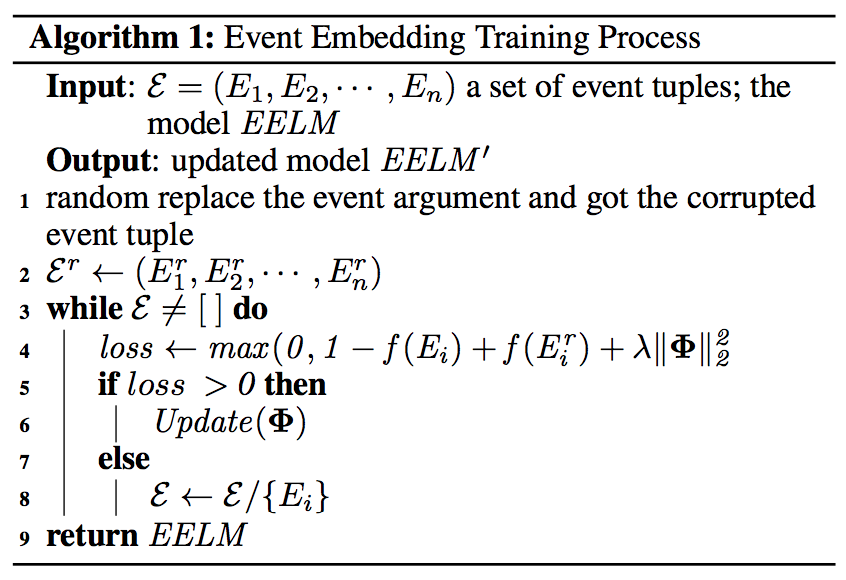
\includegraphics[scale=0.5]{img/algo1}
%   \caption{Training algorithm}
%   \hspace*{-1cm}%
% \end{figure}

% \pagebreak

\section{Baseline Code}

\begin{python}
import numpy as np
import pandas as pd

from nltk.sentiment.vader import SentimentIntensityAnalyzer
from sklearn import svm
from sklearn.model_selection import cross_val_score

data_file = "Combined_News_DJIA.csv"

def main():
  print("Importing data...")
  data = import_data("./../data/" + data_file)
  pre_processed = pre_process(data)
  sentiment_included = analyze_sentiment(pre_processed)

  train_set, test_set = split_dataset(sentiment_included)

  train_labels = ravel_labels(train_set)
  test_labels = ravel_labels(test_set)

  train_sentiments = process_sentiments(train_set)
  test_sentiments = process_sentiments(test_set)

  print("Begin Training...")
  clsfr = train(train_sentiments, train_labels.astype('int'))

  results = cross_validate(test_sentiments, test_labels.astype('int'), clsfr)

  print("Test Label Mean: " + str(test_labels.mean()))
  print("Results: " + str(results))
  print("Avg sentiment: " + str(results.mean()))

def import_data(filename):
  return pd.read_csv(filename, header=0).fillna('').values

def pre_process(data):
  # Remove the leading 'b"' in front of all lines
  print("Preprocessing...")
  for row in data[0:475]:
    for field in row[2:]:
      if field:
        field = field[1:]
  return data

def analyze_sentiment(data):
  print("Analyzing sentiment...")
  sid = SentimentIntensityAnalyzer()
  avgs = np.empty((len(data),1))
  for i in range(0,len(data)):
    sentiments = []
    for field in data[i][2:]:
      sentiments.append(sid.polarity_scores(field)['compound'])
    avg = float(sum(sentiments))/len(sentiments)
    avgs[i] = avg
  return np.append(data, avgs, axis=1)

def split_dataset(data):
  # Split 80/10/10
  n_d = len(data)
  p_train = int(n_d * 0.8)
  p_dev = p_train + int(n_d * 0.1)

  train = data[:p_train]
  dev = data[p_train:p_dev]
  test = data[p_dev:]

  print("Train: {0} / Dev: {1} / Test: {2}".format(len(train), len(dev), len(test)))

  return train, test

def train(data, labels):
  return svm.SVC(kernel='linear', C=1).fit(data, labels)

def cross_validate(data, labels, clsfr):
  return cross_val_score(clsfr, data, labels, cv=5)

def ravel_labels(data):
  return data[:,1].ravel()

def process_sentiments(data):
  return data[:,27].reshape(len(data), 1)

if __name__ == "__main__":
  main()
\end{python}


\end{document}
